\documentclass[a4paper, openany]{memoir}

\usepackage[utf8]{inputenc}
\usepackage[T1]{fontenc} 
\usepackage[english]{babel}

\usepackage{fancyhdr}
\usepackage{float}

\usepackage{amsmath}
\usepackage{amsthm}
\usepackage{amssymb}
\usepackage{enumitem}
\usepackage{multicol}
\usepackage[bookmarksopen=true,bookmarksopenlevel=2]{hyperref}
\usepackage{tikz}
\usepackage{indentfirst}

\usepackage{listings}
\usepackage{xcolor}

\pagestyle{fancy}
\fancyhf{}
\fancyhead[LE]{\leftmark}
\fancyhead[RO]{\rightmark}
\fancyhead[RE, LO]{WAD}
\fancyfoot[LE, RO]{\thepage}
\fancyfoot[RE, LO]{Pete Gautam}

\definecolor{ocre}{RGB}{52,177,201}
\definecolor{ultramarine}{RGB}{0,45,97}
\definecolor{mybluei}{RGB}{0,0,255}
\definecolor{myblueii}{RGB}{100,0,100}
\definecolor{myblueiii}{RGB}{50,234,253}

\definecolor{codegreen}{rgb}{0,0.6,0}
\definecolor{codegray}{rgb}{0.5,0.5,0.5}
\definecolor{codepurple}{rgb}{0.58,0,0.82}
\definecolor{backcolour}{rgb}{0.95,0.95,0.92}

\lstdefinestyle{mystyle}{
    backgroundcolor=\color{backcolour},   
    commentstyle=\color{codegreen},
    keywordstyle=\color{blue},
    numberstyle=\tiny\color{codegray},
    stringstyle=\color{codepurple},
    basicstyle=\ttfamily\footnotesize,
    breakatwhitespace=false,         
    breaklines=true,                 
    captionpos=b,                    
    keepspaces=true,                 
    numbers=left,                    
    numbersep=5pt,                  
    showspaces=false,                
    showstringspaces=false,
    showtabs=false,                  
    tabsize=2
}
\lstset{style=mystyle}


\lstdefinelanguage{XML}{
    sensitive=false, 
    keywords={
        xml, breakfast_menu, food, name, price, calories,
        DOCTYPE, ELEMENT, note, to, from, heading, body,
        xs, complexType, sequence, type,
        employees, employee, firstName, lastName,
    },  
    ndkeywords={},  
    morecomment=[s]{<!--}{-->},
    stringstyle=\color{purple}\ttfamily,
    morestring=[b]',
    morestring=[b]"
}

\lstdefinelanguage{JavaScript}{
  keywords={typeof, new, true, false, catch, function, return, null, try, catch, finally, switch, var, if, in, while, do, else, case, break, document, class, this, export, boolean, throw, implements, import},
  keywordstyle=\color{blue}\bfseries,
  ndkeywords={},
  ndkeywordstyle=\color{darkgray}\bfseries,
  identifierstyle=\color{black},
  sensitive=false,
  comment=[l]{//},
  morecomment=[s]{/*}{*/},
  commentstyle=\color{purple}\ttfamily,
  stringstyle=\color{red}\ttfamily,
  morestring=[b]',
  morestring=[b]"
}

\renewcommand{\headrulewidth}{1.5pt}

\chapterstyle{thatcher}
\setcounter{chapter}{1}

\begin{document}
    \chapter{The Polls App}

    \section{Creating a Django project}
    We will create a Django project called polls on PythonAnywhere. PythonAnywhere allows us to host web applications. It has an integrated bash console.

    First, we create the virtual environment \texttt{polls}. This can be done using \texttt{conda create -n polls}. Then, we create the Django project. This can be done using \texttt{django-admin startproject mysite}. In the \texttt{mysite} directory, this creates the files:
    \begin{itemize}
        \item \texttt{manage.py},
        \item \texttt{mysite/\_\_init\_\_.py},
        \item \texttt{mysite/settings.py}, 
        \item \texttt{mysite/urls.py} and 
        \item \texttt{mysite/wsgi.py}.
    \end{itemize}
    We can view the created site using the command \texttt{py manage.py runserver} in the \texttt{mysite} directory. The site looks like this right now:
    \begin{center}
        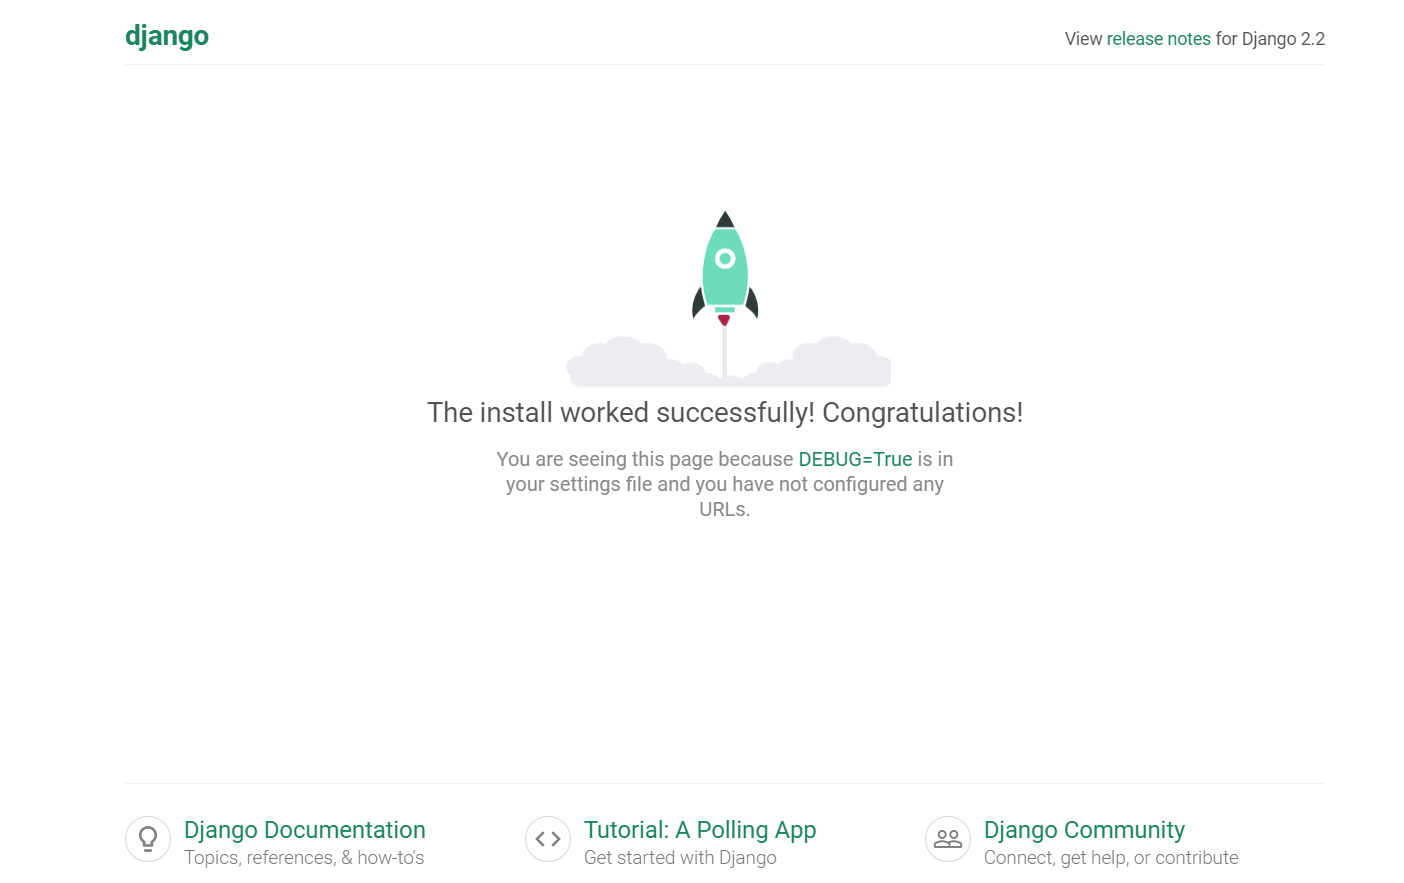
\includegraphics[scale=0.4]{src/Django1.PNG}
    \end{center}
    Next, we make the app \texttt{polls}. We can do this using \texttt{django-admin startapp polls}. This creates many files in the \texttt{mysite/polls} directory, which are: 
    \begin{itemize}
        \item \texttt{admin.py}, 
        \item \texttt{apps.py}, 
        \item \texttt{models.py}, 
        \item \texttt{views.py} and 
        \item \texttt{tests.py}
    \end{itemize}
    \newpage

    \section{Creating a view}
    In the file \texttt{views.py}, we can write views. For example, we can make this our views file to render the index page:
\begin{lstlisting}[language=python]
from django.http import HttpResponse

def index(request):
    return HttpResponse("Hello World")
\end{lstlisting}
    A view receives \texttt{HttpRequest} and returns \texttt{HttpResponse} objects. There are many ways in returning the Http response object- the one above is the simplest way.

    At this point, there is no url mapping to this view. So, we now visit the \texttt{urls.py} in the \texttt{mysite} folder to make use of the \texttt{polls} app:
\begin{lstlisting}[language=python]
from django.urls import include, path
from django.contrib import admin

urlpatterns = [
    path('polls/', include('polls.urls')),
    path('admin/', admin.site.urls)
]
\end{lstlisting}
Now, we can make use of \texttt{polls} app in the project. Next, we create another \texttt{urls.py} files in the \texttt{polls} app and register the \texttt{index} view:
\begin{lstlisting}[language=python]
from django.urls import path
from . import views

urlpatterns = [
    path('', views.index, name='index')
]
\end{lstlisting}
    Note that the \texttt{index} view now maps to \texttt{polls/}. When the url gets checked at \texttt{mysite}, we get redirected to \texttt{polls} with the empty string- this maps to the \texttt{index} view in the \texttt{polls} app. It is also possible to omit the final \texttt{/}. 

    The \texttt{path} function takes 3 parameters:
    \begin{itemize}
        \item the route, which is a URL string. We go through the urlpatterns list until we find the first matching route;
        \item the view, which is the function that django calls (when the route matches) that takes in an \texttt{HttpRequest} as an argument;
        \item the name, which allows the URL to be referenced from elsewhere unambiguously (reverse lookup). This allows for easy alternation of the URLs.
    \end{itemize}
    After the files are created and updated, we get the following webpage when we navigate to \texttt{polls}:
    \begin{center}
        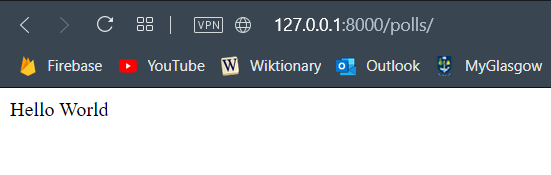
\includegraphics[scale=0.8]{src/Django2.PNG}
    \end{center}
    \newpage

    \section{Creating models}
    To initalise database setup, we run the command \texttt{py manage.py migrate}. In the file \texttt{polls/models.py}, we create the models \texttt{Question} and \texttt{Choice}:
\begin{lstlisting}[language=python]
from django.db import models

class Question(models.Model):
    question_text=models.CharField(max_length=200)
    date=models.DateTimeField("date published")

class Choice(models.Model):
    question=models.ForeignKey(Question, on_delete=models.CASCADE)
    choice_text=models.CharField(max_length=200)
    votes=models.IntegerField(default=0)
\end{lstlisting}
    A model we create has to extend the model \texttt{models.Model}. 
    Here, we have a 1-to-many relation between \texttt{Question} and \texttt{Choice}. In that case, we have the field \texttt{question} (one) in the class \texttt{Choice} (many). Moreover, we set the \texttt{on\_delete} parameter to be \texttt{models.CASCADE}- this means that when a \texttt{Question} object gets deleted, all the \texttt{Option} objects associated with that \texttt{Question} also get deleted.

    For us to make use of models in the \texttt{polls} app, we need to update the variable \texttt{INSTALLED\_APPS} in \texttt{settings.py} to include also \texttt{`polls'}. This includes the \texttt{polls} app in future database migrations. Now, we use the command \texttt{py manage.py makemigrations polls} to create these migrations. Then, we use the command \texttt{py manage.py migrate} to migrate the models.

    Next, we can manually create some data using the command \texttt{py manage.py shell}. Then, we can type the following in the command line and see their output:
\begin{lstlisting}[language=python]
>>> from polls.models import Question, Choice
>>> from django.utils import timezone
>>> ## print all the questions
>>> Question.objects.all()
<QuerySet []>
>>> ## add a question
>>> q = Question(question_text="What's new?", date=timezone.now())
>>> q.save()
>>> ## print id (the automatic primary key) and question text
>>> q.id
1
>>> q.question_text
"What's new"
>>> ## update the question text
>>> q.question_text = "What's up?"
>>> q.save()
>>> ## print all the questions
>>> Question.objects.all()
<QuerySet [<Question: Question object (1)>]>
\end{lstlisting}
    To provide a better string representation of \texttt{Question} and \texttt{Answer}, we can update our \texttt{models.py} file with \texttt{\_\_str\_\_} function:
\begin{lstlisting}[language=python]
from django.db import models

class Question(models.Model):
    question_text=models.CharField(max_length=200)
    date=models.DateTimeField("date published")
    
    def __str__(self):
        return self.question_text

class Choice(models.Model):
    question=models.ForeignKey(Question, on_delete=models.CASCADE)
    choice_text=models.CharField(max_length=200)
    votes=models.IntegerField(default=0)
    
    def __str__(self):
        return self.choice_text
\end{lstlisting}
    Now, we run \texttt{py manage.py shell} with the following in the command line:
\begin{lstlisting}[language=python]
>>> from polls.models import Question, Choice
>>> from django.utils import timezone
>>> ## print all the questions
>>> Question.objects.all()
<QuerySet [<Question: "What's up?">]>
\end{lstlisting}

    Now, we define another function \texttt{was\_published\_recently} to the \texttt{Question} model:
\begin{lstlisting}[language=python]
from datetime import timedelta

def was_published_recently(self):
    return self.date >= timezone.now() - timedelta(days=1)
\end{lstlisting}
    It returns \texttt{true} if the object was added in the last day. 

    We continue manipulating the model from the shell:
\begin{lstlisting}[language=python]
>>> from polls.models import Question, Choice
>>> from django.utils import timezone
>>> ## print all the questions
>>> Question.objects.all()
<QuerySet [<Question: "What's up?">]>
>>> ## print all the questions with id 1
>>> Question.objects.filter(id=1)
<QuerySet [<Question: "What's up?">]>
>>> ## print all the questions with id 2
>>> Question.objects.filter(id=2)
<QuerySet []>
>>> ## print all the questions starting with "What"
>>> Question.objects.filter(question_text__startswith='What')
<QuerySet [<Question: "What's up?">]>
>>> ## print the single question published this year
>>> from django.utils import timezone
>>> current_year = timezone.now().year
>>> Question.objects.get(pub_date__year=current_year)
<Question: "What's up?">
>>> ## print the single question published in 2020
>>> from django.utils import timezone
>>> current_year = timezone.now().year
>>> Question.objects.get(pub_date__year=2020)
polls.models.Question.DoesNotExist
>>> ## print the single object with id 1
>>> q = Question.objects.get(pk=1)
>>> q
<Question: "What's up?">
>>> ## check whether the question was published recently
>>> q.was_published_recently()
True
>>> ## print all the choices with question q
>>> q.choice_set.all()
<QuerySet: []>
>>> ## create choices associated with question q
>>> q.choice_set.create(choice_text="Not much", votes=0)
<Choice: "Not much">
>>> q.choice_set.create(choice_text="The sky")
<Choice: "The sky">
>>> c = Choice(question=q, choice_text="Just hacking again")
>>> c.save()
>>> c
<Choice: "Just hacking again">
>>> c.question
<Question: "What's up?">
>>> ## print all the choices with question q
>>> q.choice_set.all()
<QuerySet: [<Choice: "Not much">, <Choice: "The sky">, 
    <Choice: "Just hacking again">]>
>>> q.choice_set.count()
3
>>> ## print all the choices whose question.pub_date.year is current_year
>>> Choice.objects.filter(question__pub_date__year=current_year)
<QuerySet: [<Choice: "Not much">, <Choice: "The sky">, 
    <Choice: "Just hacking again">]>
>>> ## remove the "Just hacking again" choice
>>> c = q.choice_set.filter(choice_text__startswith="Just hacking")
>>> c
<QuerySet [<Choice: "Just hacking again">]>
>>> c.delete()
>>> ## print all the choices whose question.pub_date.year is current_year
>>> Choice.objects.filter(question__pub_date__year=current_year)
<QuerySet: [<Choice: "Not much">, <Choice: "The sky">]>
\end{lstlisting}
    Note that the function \texttt{Question.objects.filter} returns a \texttt{QuerySet} object with multiple (or none) values matching the query, while the function \newline \texttt{Question.objects.get} returns a single \texttt{Question} that satisfies the query. If there are more than one (or none) that satisfy this property, then it raises an error.

    We can create a population script to populate the database to create database content much faster. Another way of creating the content is using the django admin site. We can create a superuser using \texttt{py manage.py createsuperuser} and providing username/passsword. Then, we can navigate to the admin page. We can log in with the credentials we used previously and add/edit the models present.
    \begin{center}
        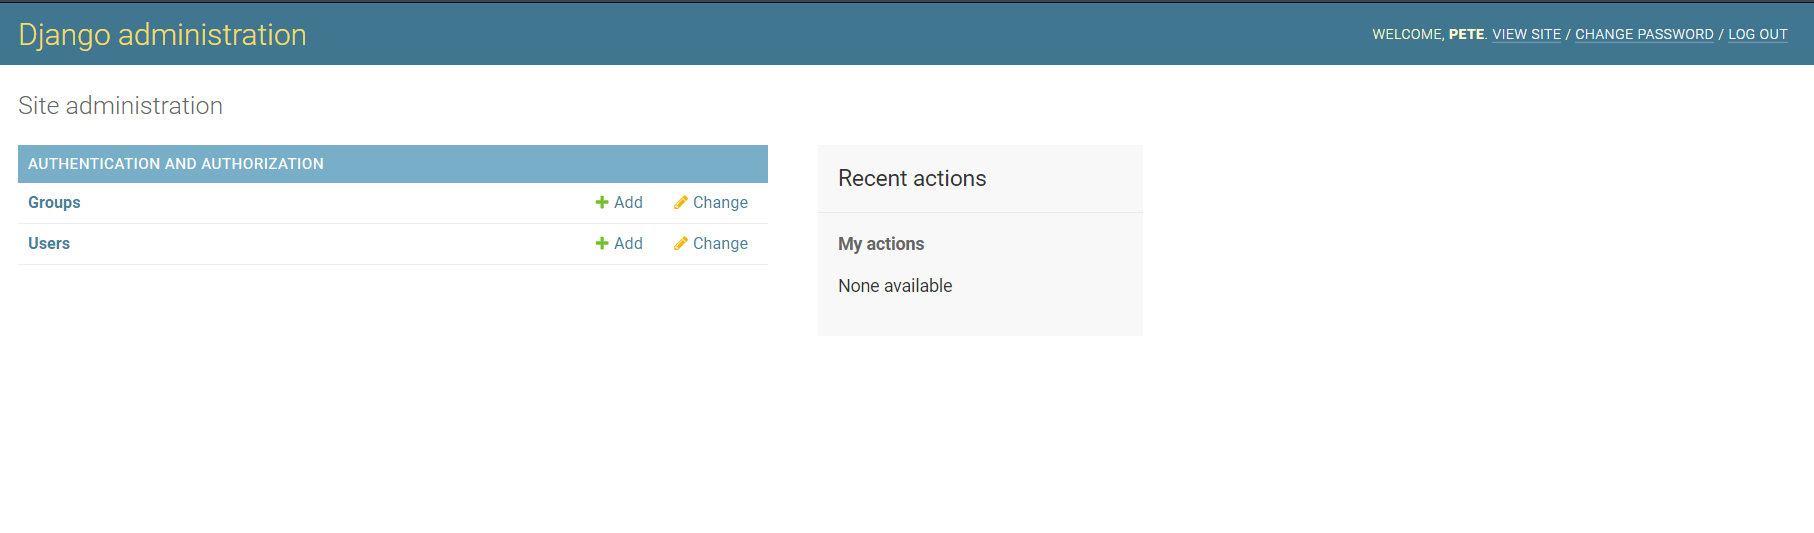
\includegraphics[scale=0.3]{src/Django3.PNG}
    \end{center}
    The models \texttt{Question} and \texttt{Choice} aren't present. To add them, we change the file \texttt{admin.py}:
\begin{lstlisting}[language=python]
from django.contrib import admin
from .models import Question, Choice

admin.site.register(Question)
admin.site.register(Choice)
\end{lstlisting}
    Then, after we reload the webpage, we get the two models:
    \begin{center}
        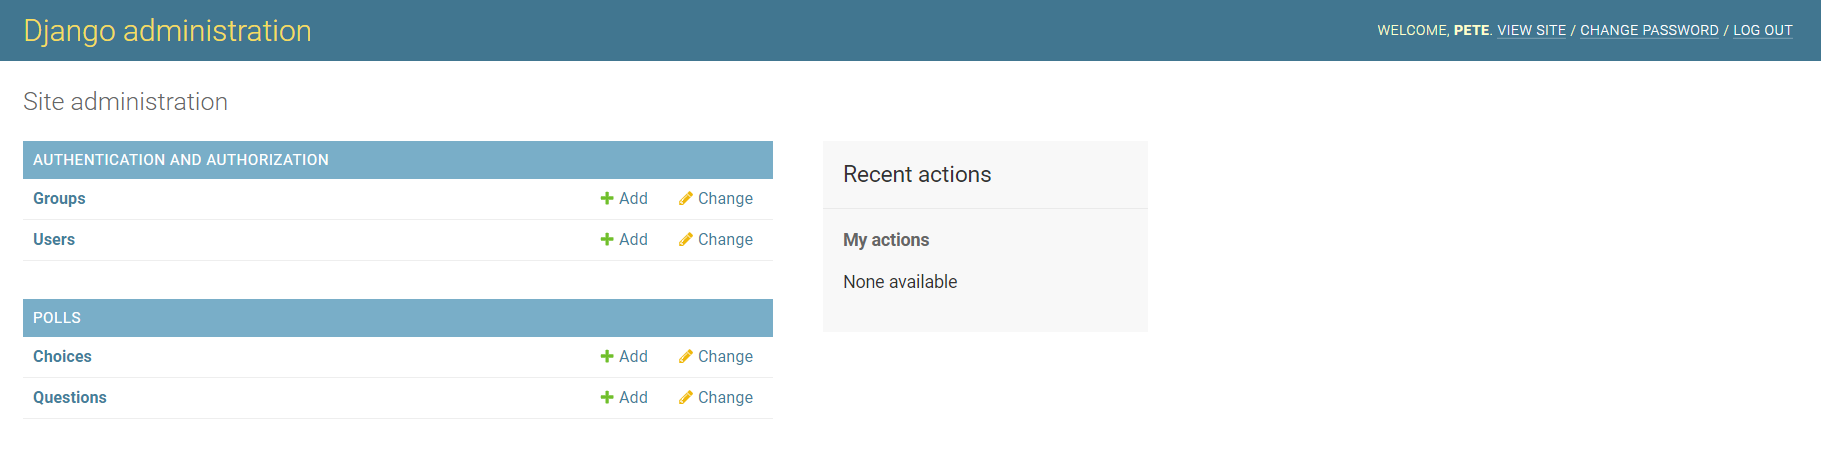
\includegraphics[scale=0.3]{src/Django4.PNG}
    \end{center}
    We can browse the objects we have created by clicking on the relevant model. For example, the \texttt{Choice} objects we had are:
    \begin{center}
        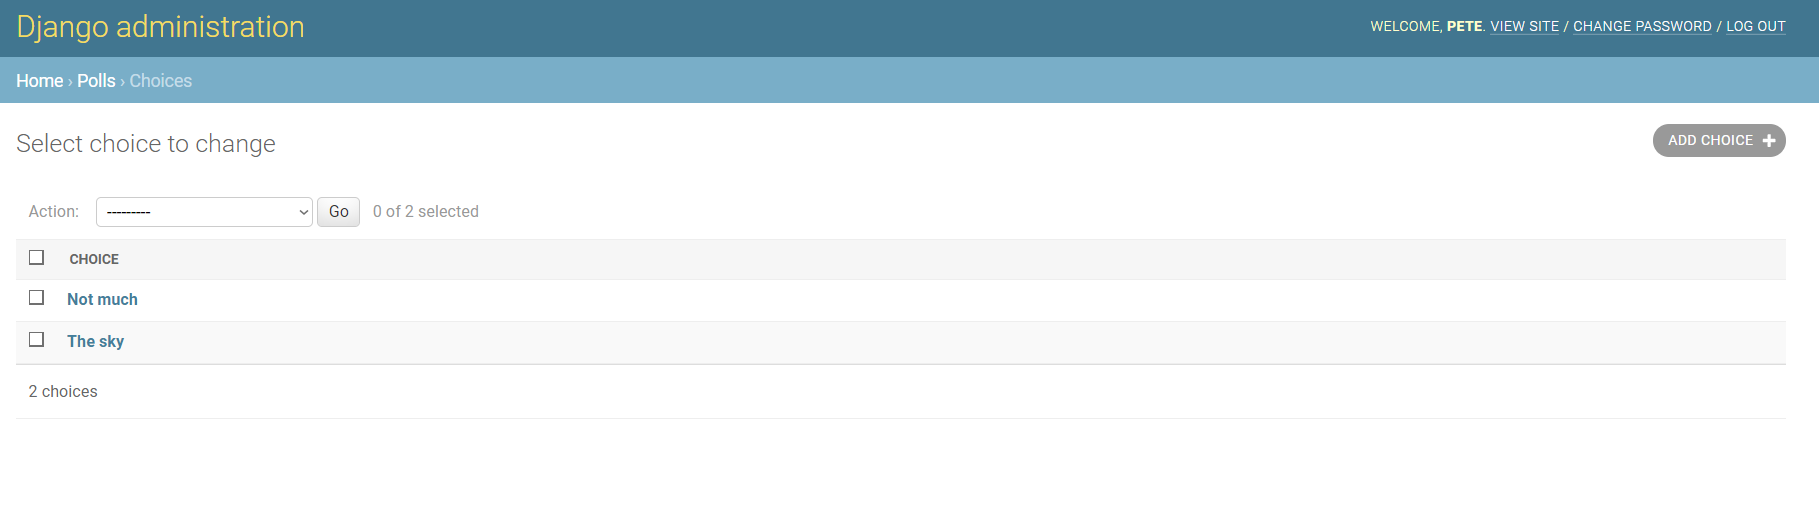
\includegraphics[scale=0.3]{src/Django5.PNG}
    \end{center}
    We can also edit/create another \texttt{Choice} object. For example, if we wanted to edit \texttt{"Not much"}, we would get:
    \begin{center}
        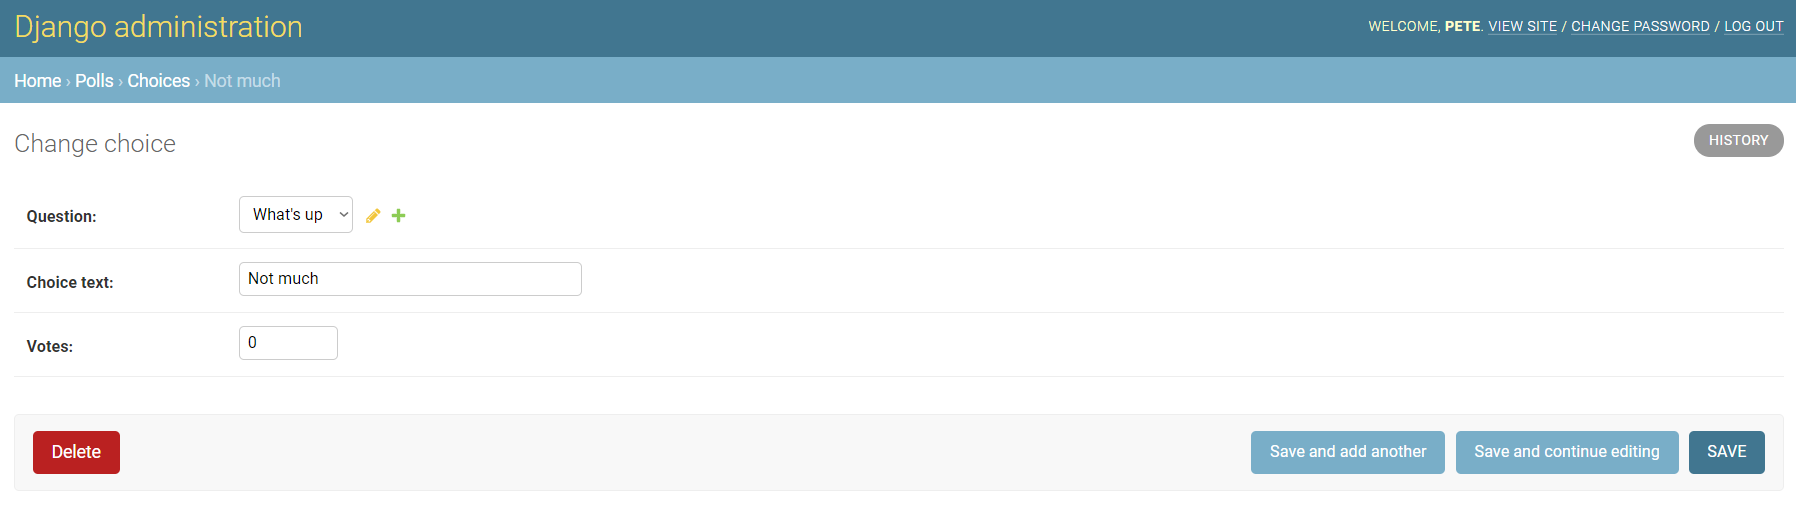
\includegraphics[scale=0.3]{src/Django6.PNG}
    \end{center}
    \newpage

    \section{Creating more views}
    We now add more views to \texttt{views.py}
\begin{lstlisting}[language=python]
from django.http import HttpResponse

def index(request):
    return HttpResponse("Hello World")

def detail(request, question_id):
    response = "You're looking at question %s"
    return HttpResponse(response % question_id)

def results(request, question_id):
    response = "You're looking at the results of question %s"
    return HttpResponse(response % question_id)
    
def vote(request, question_id):
    response = "You're voting on question %s"
    return HttpResponse(response % question_id)
\end{lstlisting}
    This is not the final look of the page- we are just creating the pages.

    Then, we update the file \texttt{urls.py} in the \texttt{polls} app:
\begin{lstlisting}[language=python]
from django.urls import path
from . import views

urlpatterns = [
    ## /polls/
    path('',views.index,name='index'),
    ## e.g. /polls/3
    path('<int:question_id>/',views.detail,name='detail'),
    ## e.g. /polls/3/results
    path('<int:question_id>/results/',views.results,name='results')
    ## e.g. /polls/3/vote
    path('<int:question_id>/vote/',views.vote,name='vote')
]
\end{lstlisting}
    We make use of \texttt{<int:question\_id>} to allow any integer to pass in. This integer also becomes the second parameter of the view function.

    Next, we are now going to change the \texttt{index} view so that it returns the latest 3 questions:
\begin{lstlisting}[language=python]
from .models import Question

def index(request):
    ## find the latest 3 questions
    latest_questions = Question.objects.order_by('-date')[:3]
    ## present it in a clear string and return it
    output = ", ".join([q.question_text for q in latest_question])
    return HttpResponse(output)
\end{lstlisting}
    We will now add a second question \texttt{Question 2}. Then, the index page looks like:
    \begin{center}
        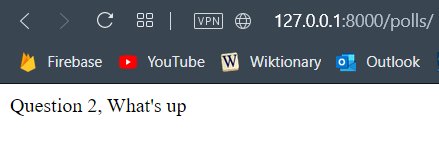
\includegraphics[scale=0.7]{src/Django7.PNG}
    \end{center}
    The issue with rendering views like this is that they are all hard-coded within the view functions. They should only deal with logic; a template should handle any views. So, we create the template \texttt{mysite/templates/polls/index.html}:
\begin{lstlisting}[language=html]

    <ul>
        
            <li><a href="/polls/{{ question.id }}/">
                {{ question.question_text }}
            </a></li>
        
    </ul>

    <p>No polls are available</p>

\end{lstlisting}
    A Django template file is composed of html tags, as well as variables (e.g. \texttt{\{\{  variable \}\}}) and logic (e.g. \texttt{\{\% logic \%\}}). To register templates, we need to add to the \texttt{settings.py} file the statement 
\begin{lstlisting}[language=python]
TEMPLATE_DIR = os.path.join(BASE_DIR, 'templates')
\end{lstlisting}
    and update the variable \texttt{TEMPLATES} accordingly. Finally, we update the function \texttt{index} in \texttt{views.py}:
\begin{lstlisting}[language=python]
from django.shortcuts import render

def index(request):
    ## find the latest 3 questions
    latest_questions = Question.objects.order_by('date')[:3]
    context_dict = {'latest_questions_list': latest_questions}
    return render(request, 'polls/index.html', context_dict)
\end{lstlisting}
    The render function returns an HttpResponse object that uses the template provided along with the context dictionary. Now, the index page looks like:
    \begin{center}
        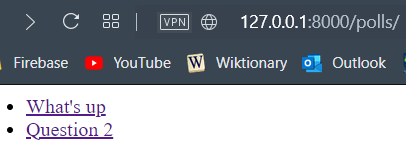
\includegraphics[scale=0.7]{src/Django8.PNG}
    \end{center}
    At this point, clicking on any of the question shows a very basic details page. Now, we will use the \texttt{question\_id} to render content specific to that question. However, it is possible that there is no question with the id provided. In that case, we need to redirect to 404 page. So, we update the details view as follows:
\begin{lstlisting}[language=python]
from django.http import Http404

def detail(request, question_id):
    try:
        question = Question.objects.get(pk=question_id)
    except Question.DoesNotExist:
        raise Http404("Question does not exist!")
    context_dict = {'question': question}
    return render(request, 'polls/detail.html', context_dict)
\end{lstlisting}
    There is a shortcut to doing this:
\begin{lstlisting}[language=python]
from django.shortcuts import get_object_or_404

def detail(request, question_id):
    question = get_object_or_404(Question, pk=question_id)
    context_dict = {'question': question}
    return render(request, 'polls/detail.html', context_dict)
\end{lstlisting}
    Next, we create the template \texttt{detail.html}:
\begin{lstlisting}[language=html]
<h1>{{ question.question_text }}</h1>
<ul>
    
        <li>{{ choice.choice_text }}</li>
    
</ul>
\end{lstlisting}
    Then, the details page looks like:
    \begin{center}
        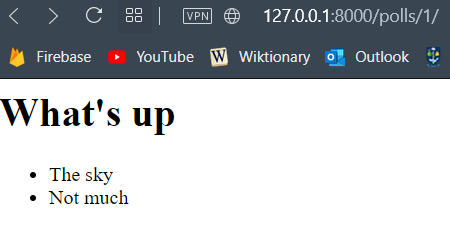
\includegraphics[scale=0.7]{src/Django9.PNG}
    \end{center}
    When we wrote the link to a question in \texttt{index} template, the link was partially hardcoded. This becomes challenging to change URLs on projects with many templates. We resolve this using the name argument in \texttt{urls.py} together with the \texttt{\{\% url \%\}} tag. So, the \texttt{index.html} template becomes:
\begin{lstlisting}[language=python]

    <ul>
        
            <li><a href="">
                {{ question.question_text }}
            </a></li>
        
    </ul>

    <p>No polls are available</p>

\end{lstlisting}
    We have only changed line 4. To namespcace the URL names to differentiate between the apps, we need to add \texttt{app\_name = 'polls'} to \texttt{polls/urls.py}. Also, we need to replace \texttt{'detail'} in line 4 of the code above to \texttt{'polls:detail'}.
    \newpage

    \section{Creating a form}
    Next, we update the details page to allow users to vote in a poll. First, we update the template \texttt{detail.html}:
\begin{lstlisting}[language=html]
<h1>{{ question.question_text }}</h1>


    <p><strong>{{ error_message }}</strong></p>


<form action="" method="POST">
    
    <div>
        
            <div>
                <input type="radio" name="choice" 
                    id="choice {{ forloop.counter }}" 
                    value="{{ choice.id }}">
                <label for="choice {{ forloop.counter }}">
                    {{ choice.choice_text }}
                </label>
            </div>
        
    </div>
    <input type="submit" value="Vote">
</form>
\end{lstlisting}
    The post action is to \texttt{vote} function. Next, we update the functions \texttt{vote} and \texttt{results}:
\begin{lstlisting}[language=python]
from django.urls import reverse
from .models import Choice
from django.http import HttpResponseRedirect

def vote(request, question_id):
    question = get_object_or_404(Question, pk=question_id)
    try:
        selected_choice = question.choice_set.get(
            pk=request.POST['choice'])
    except (KeyError, Choice.DoesNotExist):
        context_dict = {
            'question': question,
            'error_message': "You didn't select a choice"
        }
        return render(request, 'polls/detail.html', context_dict)
    else:
        selected_choice.votes += 1
        selected_choice.save()
        
        return HttpResponseRedirect(reverse('polls:results', 
            args=(question.id,)))

def results(request, question_id):
    question = get_object_or_404(Question, pk=question_id)
    context_dict = {'question': question}
    return render(request, 'polls/results.html', context_dict)
\end{lstlisting}
    The \texttt{reverse} function stops us from hard-coding urls in python code. Then, we create the template \texttt{results.html}:
\begin{lstlisting}[language=html]
<h1>{{ question.question_text }}</h1>

<ul>
    
        <li>{{ choice.choice_text }} -- {{ choice.votes }} 
            vote{{ choice.votes|pluralize}}</li>
    
</ul>

<a href="">Vote again</a>
\end{lstlisting}
    The \texttt{pluralize} adds an \texttt{s} if appropriate. Now, if we vote in the details page without selecting an option, we get the following response:
    \begin{center}
        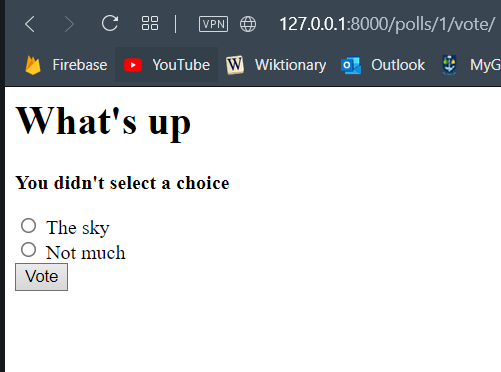
\includegraphics[scale=0.7]{src/Django10.PNG}
    \end{center}
    Instead, if we vote for one of the choices, we get the following response:
    \begin{center}
        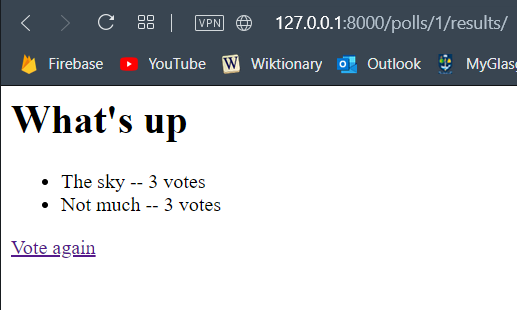
\includegraphics[scale=0.7]{src/Django11.PNG}
    \end{center}
    \newpage

    \section{Creating the population script}
    We will now create a population script that sets up the initial database. To do so, we create the file \texttt{mysite/populate\_polls.py}. The content within the file is:
\begin{lstlisting}[language=python]
import os
os.environ.setdefault('DJANGO_SETTINGS_MODULE', 'mysite.settings')

import django
django.setup()

from polls.models import Question, Choice
from datetime import datetime
from pytz import utc

def populate():
    ## delete pre-existing data
    Question.objects.all.delete()
    Choice.objects.all.delete()
    
    ## question 1
    question1_choices = [
        {
            'choice_text': "The sky",
            'votes': 5
        },
        {
            'choice_text': "Just hacking",
            'votes': 8
        },
        {
            'choice_text': "Not much",
            'votes': 2
        }
    ]
    
    ## similarly for questions 2-5  ...
    
    question = {
        "What's up?": {
            "choices": question1_choices,
            "date": datetime(2020, 10, 17, 15, 30, tzinfo=utc)
        },
        ## similarly for questions 2-5 ...
    }
    
    for question, question_data in question.items():
        q = add_question(question, question_data["date"])
        for c in question_data["choices"]:
            add_choice(q, c["choice_text"], c["votes"])

def add_question(question_text, pub_date):
    question = Question.objects.get_or_create(question_text=question_text, date=date)[0]
    question.save()
    return question

def add_choice(question, choice_text, votes):
    choice = Choice.objects.get_or_create(question=question, choice_text=choice_text, votes=votes)[0]
    choice.save()
    return choice

## Execution starts here
if __name__ == '__main__':
    populate()
\end{lstlisting}
    To run the script, we run \texttt{py manage.py}. We might need to makemigrations and migrate to run this.
    \newpage

    \section{Creating tests}
    Tests are simple routines that check the operation of your code. Testing operates at different levels. With automated tests, the testing work is done by the system. We create a set of tests once. As we make changes to our app, we can check the code still works as we originally intended.

    Tests save us time. Tests do not just identify the problems. They also help us prevent them. Tests make the code more attractive (to others). Also, tests help teams work together.

    In test-driven development, we write a test before coding. It might seem counter-intuitive, but it is similar to what we do already. We describe a problem and create some code to solve it. Test-driven development formalises the problem in a Python test case. It is easier to write tests as we create the code rather than later.

    The polls app already has a bug! The function \texttt{was\_published\_recently} in the class \texttt{Question} within \texttt{models.py} is supposed to return \texttt{True} if it was published in the last day. However, it returns \texttt{True} even if the \texttt{date} is in the future.

    Now, we add to the file \texttt{tests.py} to expose the bug:
\begin{lstlisting}[language=python]
from datetime import timedelta

from django.utils import timezone
from django.test import TestCase
from .models import Question

class QuestionMethodTests(TestCase):
    def test_was_published_recently_with_future_question(self):
        ## was_published_recently() should return False for
        ## questions whose publication date is in the future
        time = timezone.now() + timedelta(days=30)
        future_question = Question(date=time)
        self.assertIs(future_question.was_published_recently(), 
            False)
\end{lstlisting}
    We can run this file using the command \texttt{py manage.py test polls.test}. This test will fail because the function returns \texttt{True}. Testing makes use of a dummy database for each class; it does not affect the pre-existing database.

    When we call \texttt{py manage.py test polls.test}, Django found a subclass of \texttt{django.test.TestCase}. It then created a special database for the purpose of testing. It then looks for test methods. These are the methods whose name begins with test. The \texttt{test\_was\_published\_recently\_with\_future\_question} test created a \texttt{Question} whose \texttt{date} was 30 days in the future. Using the method \texttt{assertIs}, we then discovered that it returned \texttt{True} when we called the method \texttt{was\_published\_recently}, even though we wanted it to return \texttt{False}. 

    Now, we will fix the bug in \texttt{models.py}:
\begin{lstlisting}[language=python]
def was_published_recently(self):
    now = timezone.now()
    return now - timedelta(days=1) <= self.date <= now
\end{lstlisting}
    This passes the test. We can now add more tests:
\begin{lstlisting}[language=python]
from datetime import timedelta

from django.utils import timezone
from django.test import TestCase
from .models import Question

class QuestionMethodTests(TestCase):
    def test_was_published_recently_with_future_question(self):
        ## was_published_recently() should return False for
        ## questions whose publication date is in the future
        time = timezone.now() + timedelta(days=30)
        future_question = Question(date=time)
        self.assertIs(future_question.was_published_recently(), 
            False)
    
    def test_was_published_recently_with_old_question(self):
        ## was_published_recently() should return False for
        ## questions whose publication date is older than 1 day.
        time = timezone.now() - timedelta(days=30)
        future_question = Question(date=time)
        self.assertIs(future_question.was_published_recently(), 
            False)
    
    def test_was_published_recently_with_recent_question(self):
        ## was_published_recently() should return False for
        ## questions whose publication date is within the last day.
        time = timezone.now() - timedelta(hours=1)
        future_question = Question(date=time)
        self.assertIs(future_question.was_published_recently(), 
            True)
\end{lstlisting}
    This still passes the test.

    \subsection{Testing Views}
    Django provides a test \texttt{Client} to simulate a user interacting with the code at the view level. We can use \texttt{Client} in \texttt{tests.py} or in the shell. We start by using the shell:
\begin{lstlisting}[language=python]
>>> from django.test.utils import setup_test_environment
>>> from django.test import Client
>>> setup_test_environment()
>>> client = Client()
>>> response = client.get("/")
Not Found: /
>>> response.status_code
404
>>> from django.urls import reverse
>>> response = client.get(reverse('polls:index'))
>>> response.status_code
200
>>> response.context['latest_questions_list']
<QuerySet [<Question: "What's up">]>
\end{lstlisting}
    The content here will be operated on the same database unlike before since it is through the command line. Now, we update the file \texttt{tests.py}:
\begin{lstlisting}[language=python]
from django.shortcuts import reverse

def create_question(question_text, days):
    ## creates a question given question_text and 
    ## published the given number of days offset to now
    ## (negative for past, positive for future)
    time = timezone.now() + timedelta(days=days)
    return Question.objects.create(question_text=question_text, 
        date=time)

class QuestionViewTest(TestCase):
    def test_index_view_with_no_questions(self):
        ## If no questions exist, an appropriate message
        ## should be displayed
        response = self.client.get(reverse('polls:index'))
        self.assertEqual(response.status_code, 200)
        self.assertContains(ressponse, "No polls are available.")
        self.assertQuerySetEqual(response.context
            ['latest_questions_list'], [])
    
    def test_index_with_a_past_question(self):
        ## Only past questions published should be displayed
        create_question(question_text="Past Question", days=-30)
        response = self.client.get(reverse('polls:index'))
        self.assertQuerySetEqual(request.context
            ['latest_question_list'], ['<Question: Past Question'])
    
    def test_index_with_a_future_question(self):
        # Future questions should not be displayed
        create_question(question_text="Future Question", days=30)
        response = self.client.get(reverse('polls:index'))
        self.assertContains(ressponse, "No polls are available.")
        self.assertQuerySetEqual(response.context
            ['latest_questions_list'], [])
    
    ## ... more tests
\end{lstlisting}
    We can add more tests similar to those already present. We could also improve our application in other ways, while adding tests to check those features. For example, we could ensure that questions cannot be published without choices. Our views could check this, and exclude such questions. Our tests would create a question without choices and then test that it's not published. Also, perhaps logged-in admin users should be allowed to see unpublished questions, but not ordinary visitors. Again, whatever needs to be added to the software to accomplish this should be accompanied by a test. Having too many tests is not an issue.

    We might need to update the test, e.g. if we amend our views so that only questions with choices are published. It doesn't matter if tests are redundant. Tests should be arranged so that they are manageable. There should be a separate TestClass for each model or view. We should also have a separate test method for each set of conditions we want to test. We should give test methods intuitive names that describe their function.
    \newpage

    \section{Static Files}
    Static files correspond to images, JavaScript and CSS. We will now add a stylesheet (via a CSS file) and an image. We create a file at \texttt{static/polls} \texttt{/style.css} inside \texttt{polls} folder with the following CSS code:
\begin{lstlisting}
li a {
    color: green;
}
\end{lstlisting}
    To make use of static files in our templates, the top line should be \texttt{\{\% load staticfiles \%\}}. We also update the \texttt{settings.py} file with:
\begin{lstlisting}[language=python]
STATIC_DIR = os.path.join(BASE_DIR, 'static')
STATICFILES_DIRS = [STATIC_DIR, ]
\end{lstlisting}
    so that static files are hosted. Then, the final version of the project is:
    \begin{center}
        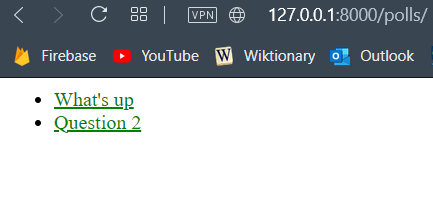
\includegraphics[scale=0.6]{src/Django12.PNG}
    \end{center}

\end{document}